\begin{table}
\caption{Overview of assimilation experiments performed.}
\centering
\begin{tabular}{p{2cm}p{2cm}p{6cm}p{4cm}}
	Number & Model &  Assimilated Quantities  & Run dates \\
\hline
1 & WACCM &	none   & 1 Oct 2009 - 31 Mar 2010	\\
2 & WACCM &	GPS-RO + NNRA$^a$ tropics only & 1 Oct 2009 - 31 Mar 2010	\\
3 & WACCM &	GPS-RO + NNRA$^a$ whole atmosphere  & 1 Oct 2009 - 31 Mar 2010	\\
4 & CAM	&	none &  1 Jan - 28 Feb 2009 \\
5 & CAM &	$\chi_1$, $\chi_2$, $\chi_3$ & 1 Jan - 28 Feb 2009 \\
6 & CAM &	Temperature	& 1 Jan -31 Jan 2009	\\
7 & CAM &	Temperature, $\chi_1$, $\chi_2$, $\chi_3$ & 1 Jan - 17 Jan 2009\\
\hline
\end{tabular}
\tablenotetext{a}{Observations used in the NCEP/NCAR Reanalysis project \citet{Saha2010}, which include radiosonde and aircraft winds and temperatures, plus satellite drift winds.}
\label{tab:expts}
\end{table}
\clearpage



%------comparison of the DA runs in the observation space
\begin{figure}[p]
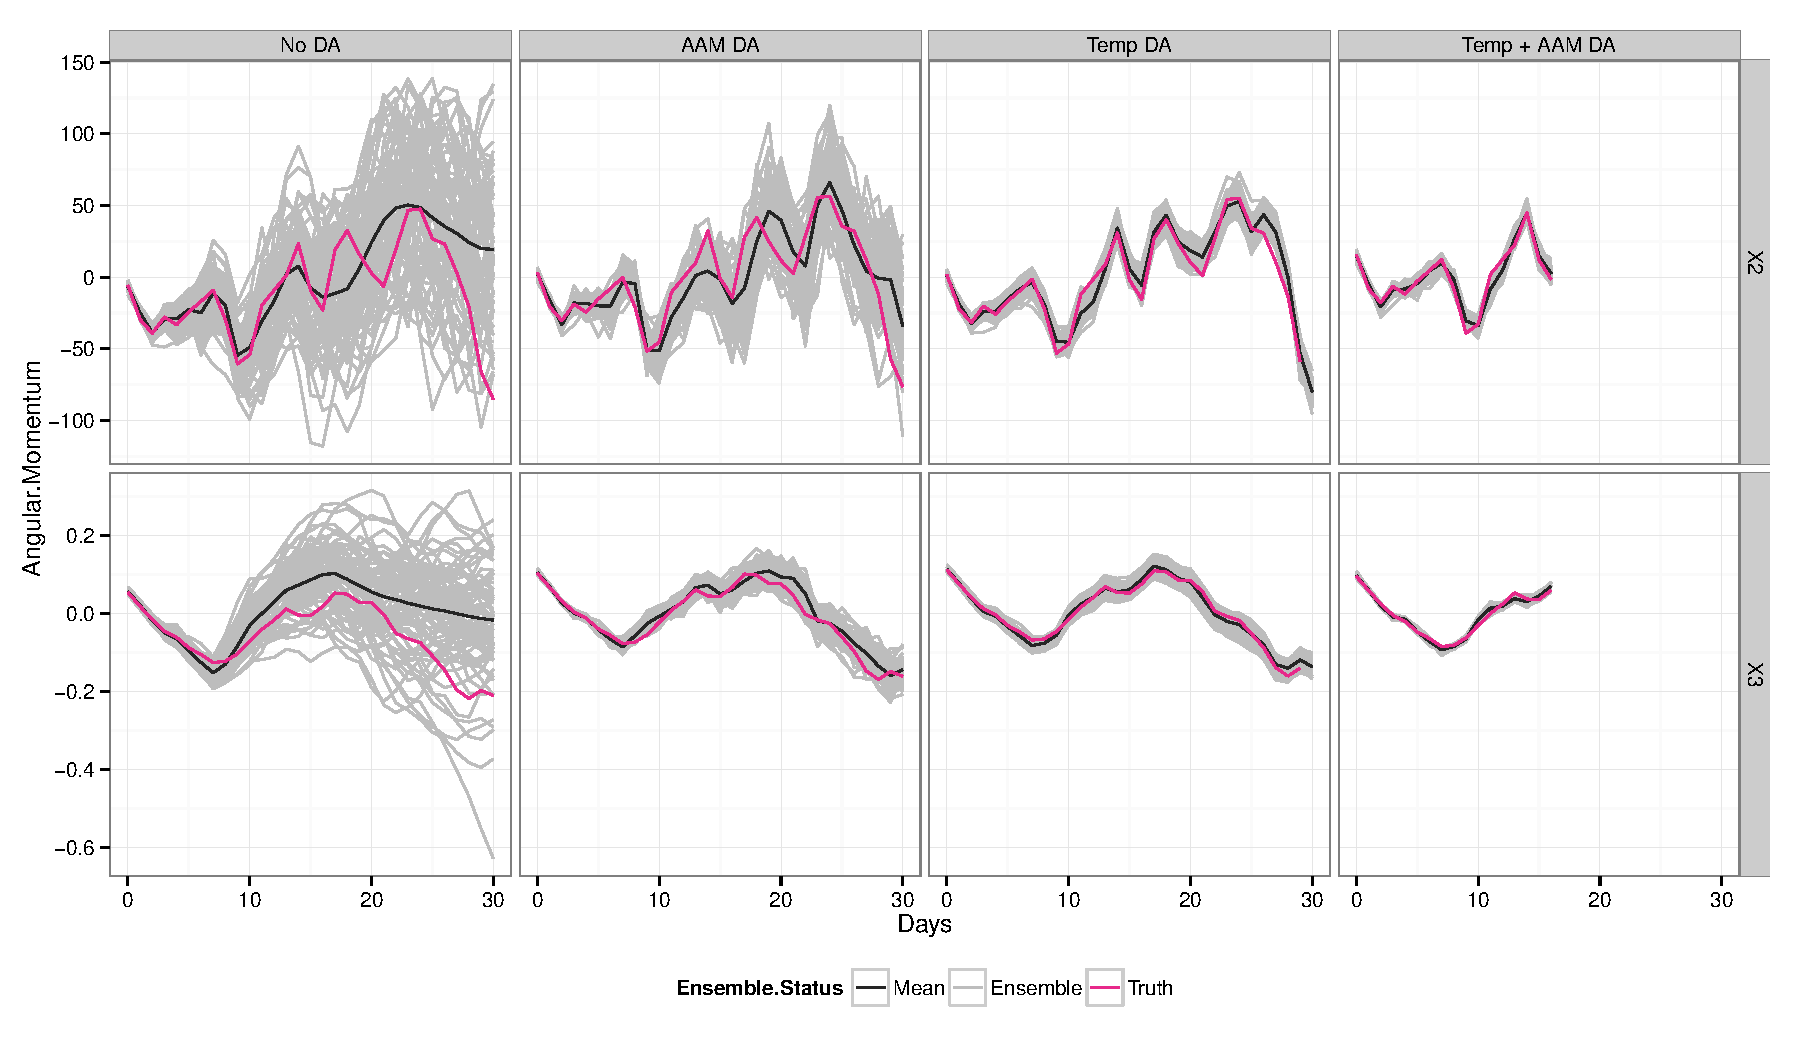
\includegraphics[width=\textwidth]{Paper_figures/ERPDA_paper_erpda_obs_space.pdf} 
\caption{ The DART-CAM prior ensemble (gray) and its mean (black) compared to the true state (pink) in terms of angular momentum components $\chi_2$ and $\chi_3$, comparing four perfect-model experiments with DART-CAM (see text and Table \ref{tab:expts}).  }
 \label{fig:fit_to_ERPs}
\end{figure}

%-----evolution of the covariances between local variables and the AAM observations 
 \begin{figure}
	 \includegraphics[width=\textwidth]{Paper_figures/ERPDA_paper_U_to_LOD_covariances.pdf}
	 \caption{Snapshots of the covariance between the zonal wind and the axial angular momentum ($\chi_3$) shortly after spin-up (top row), at the end of the assimilation period (middle row), and averaging over the entire period minus spinup time (bottom row), assimilatng only the angular momentum. The lefthand column shows snapshots at 320 hPa; the righthand column shows snapshots at 10 hPa.}
 \label{fig:covariances}
\end{figure}

%-----evolution of the prior error and corresponding increments 
 \begin{figure}
	 \includegraphics[height=0.9\textheight]{Paper_figures/ERPDA_paper_U_priorerror_vs_increment_vs_ER_30jan_strattrop.pdf}
	 \caption{Snapshots of the 320 hPa zonal wind (a) true error (true minus prior ensemble mean), (b) analysis increment (posterior minus prior ensemble mean), (c) square error reduction (posterior minus prior mean square error), and (d) reduction in the ensemble spread (posterior minus prior, scaled as in (\ref{eq:EvsS})). All plots are shown for 30 Jan, for the CAM ensemble assimilating only atmospheric angular momentum. } 
 \label{fig:error_increments}
\end{figure}

%-----focus on the ensemble in two regions to show how it is moved away from the true state
 \begin{figure}
	 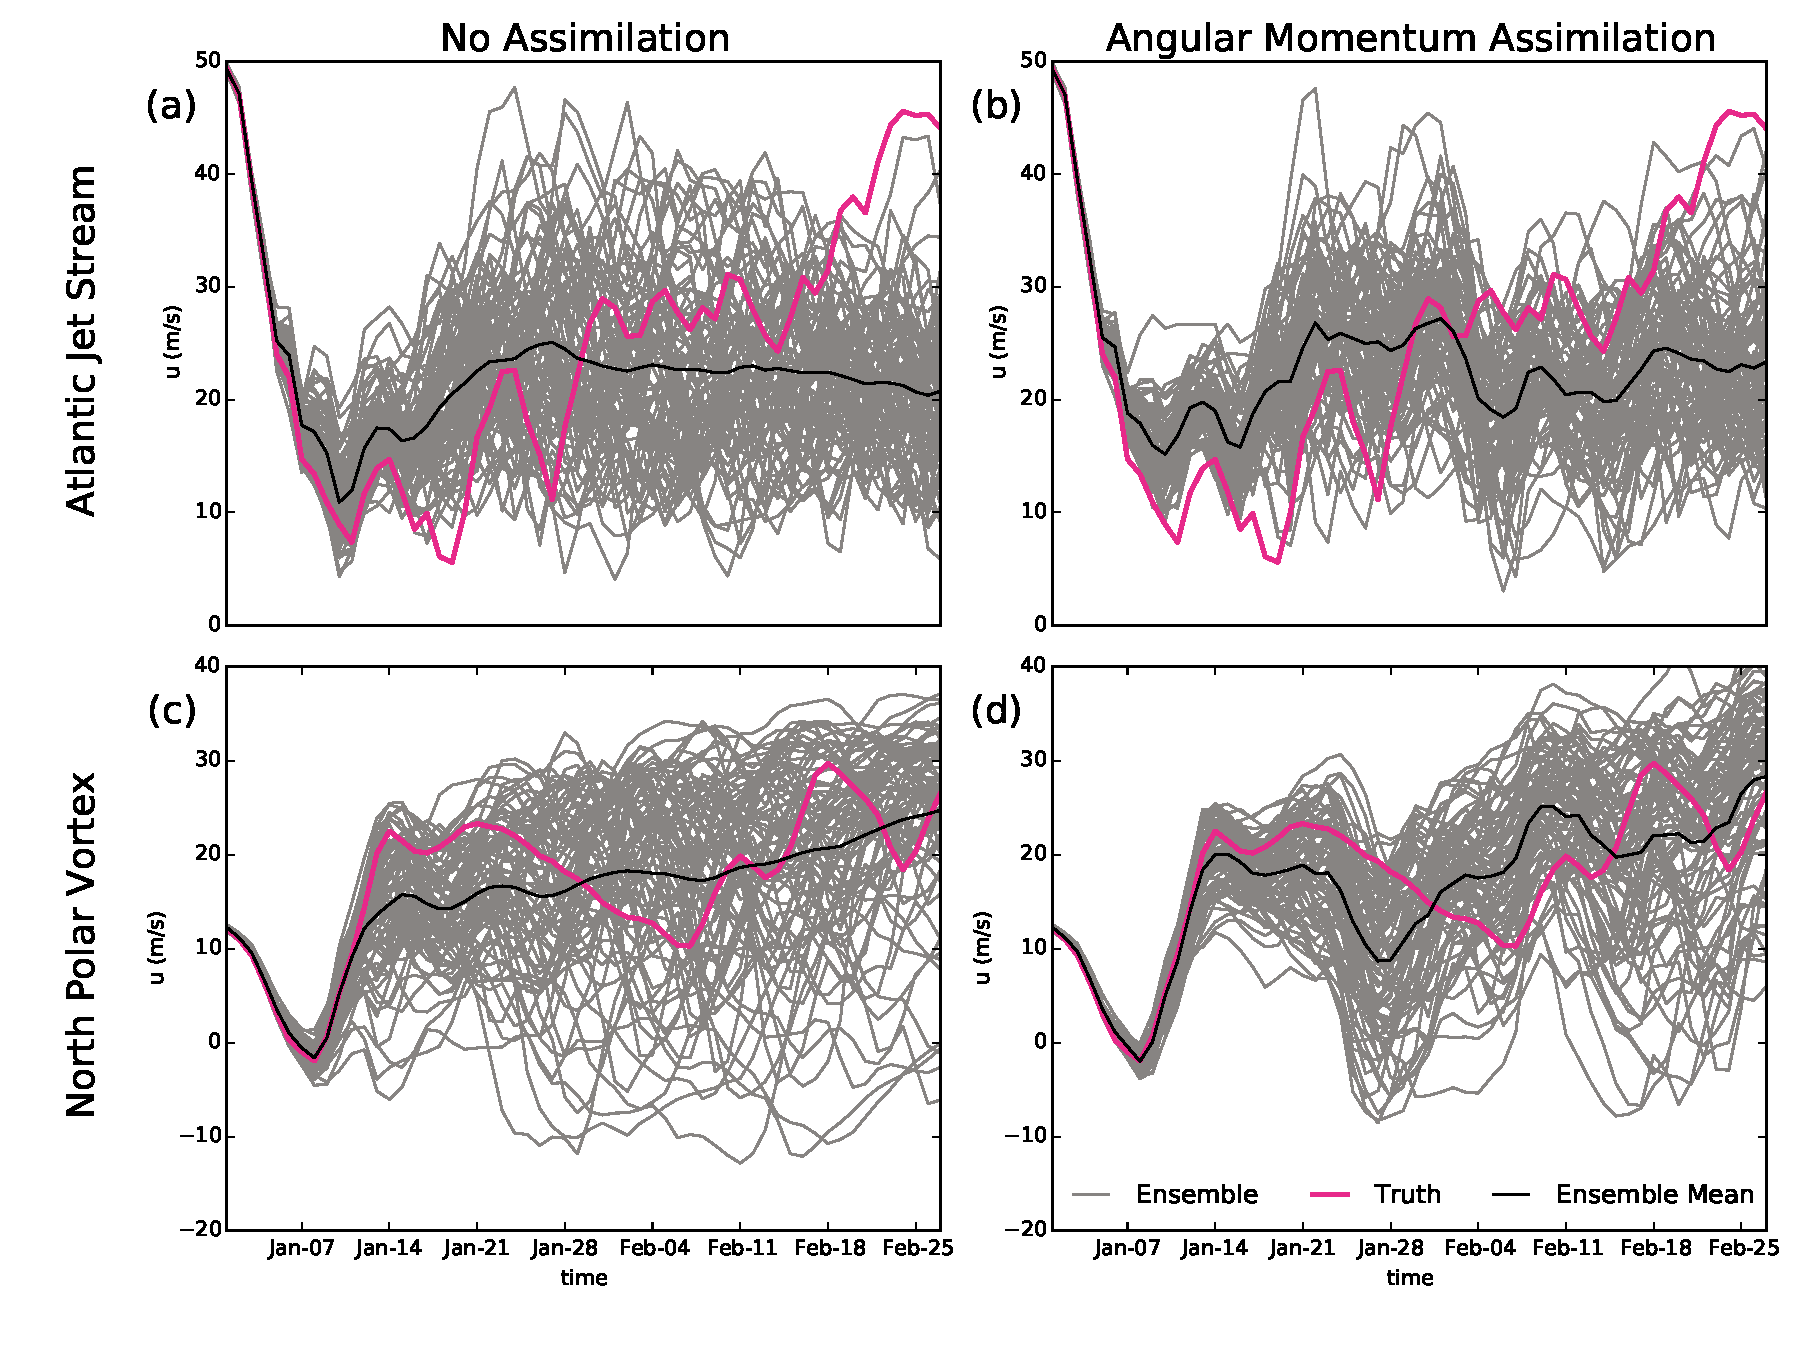
\includegraphics[width=\textwidth]{Paper_figures/ERPDA_paper_point_checks.pdf}
	 \caption{Comparison of the ensemble and its mean to the true state, comparing no assimilation (left column), and assimilation of the three angular momentum components (right column). The top row shows zonal wind averaged over the Atlantic jet stream, and the bottom row shows zonal wind averaged in the polar vortex (see text).}
	 \label{fig:point_checks}
\end{figure}


%------MSE diff between ERPRST and RST (red is good)
 \begin{figure}
	 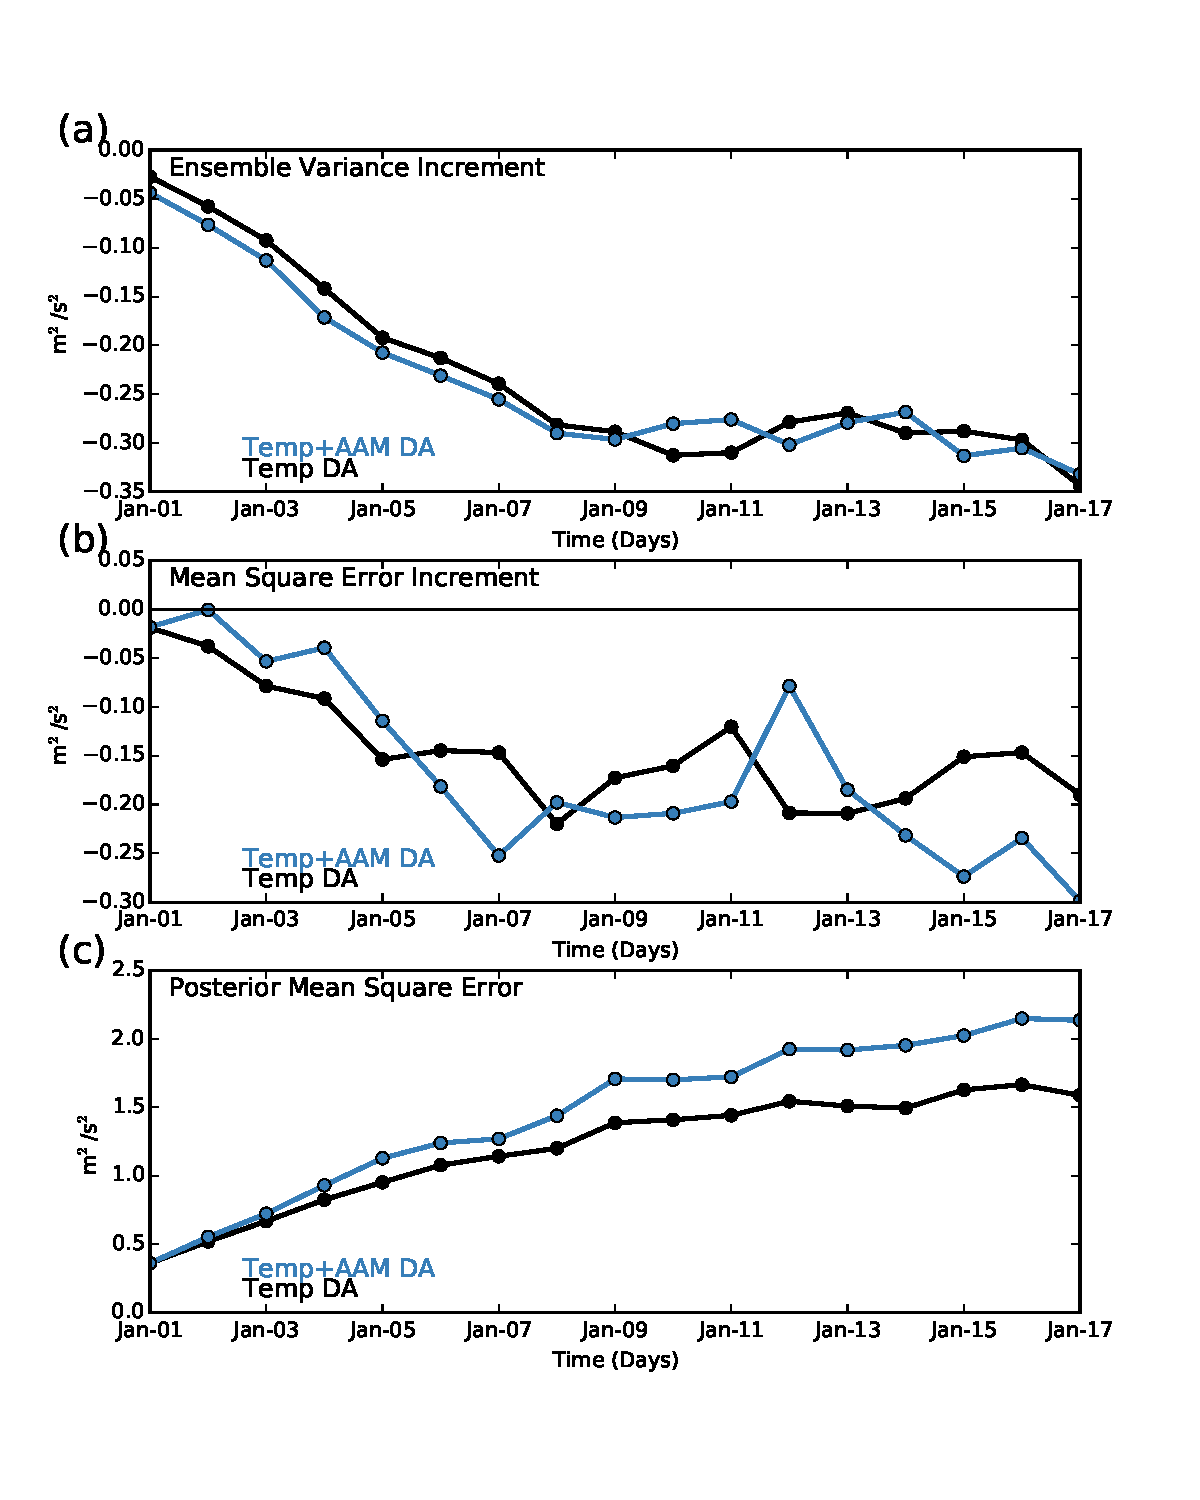
\includegraphics[width=0.7\textwidth]{Paper_figures/ERPDA_paper_MSE_RST_vs_ERPRST_global.pdf}
	 \caption{(a) Global average increment (posterior-prior) in the ensemble variance, scaled as in (\ref{eq:EvsS}), for zonal wind in a DART-WACCM ensemble assimilating local temperatures (black) and temperatures along with atmospheric angular momentum (blue). (b) As in (a), but for the increment in the mean square error. (c) As above, but showing the absolute posterior mean square error.}
	 \label{fig:added_value_MSE}
\end{figure}

%-------comparison of the WACCM experiments in terms of true error ----
 \begin{figure}
	 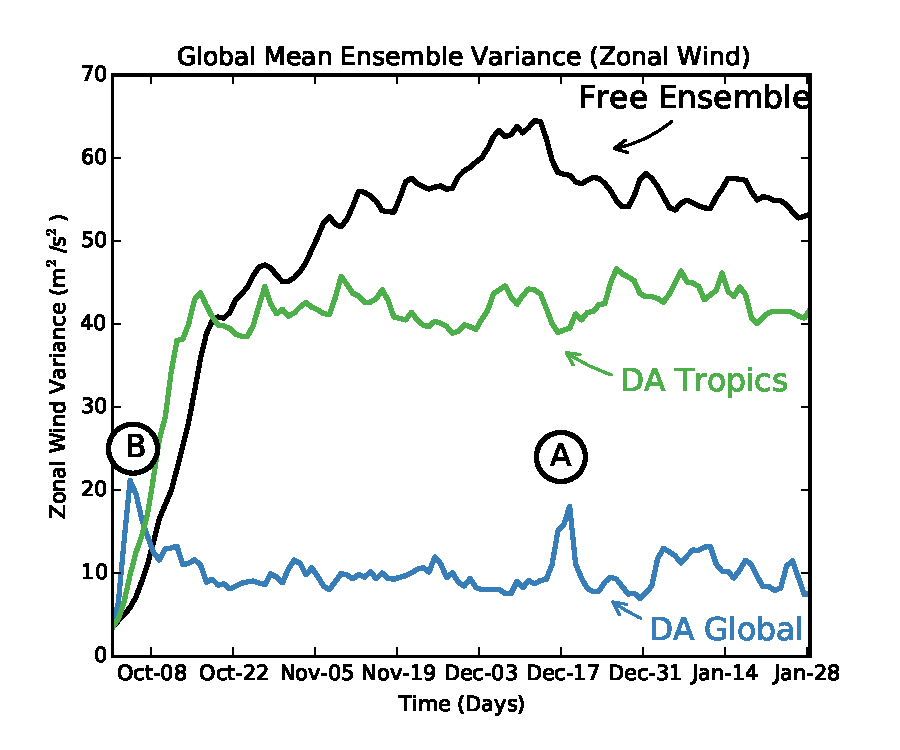
\includegraphics[width=\textwidth]{Paper_figures/ERPDA_paper_evalvariable_state_space.pdf}
	 \caption{Global-average ensemble variance in the zonal wind as a function of time, comparing a DART-WACCM with no assimilation, and with 6-hourly assimilation of meteorolgical observations (see text).}
	 \label{fig:evalvariable_state}
\end{figure}
%-------comparison of the WACCM experiments in terms of aam ----
\begin{figure}
	 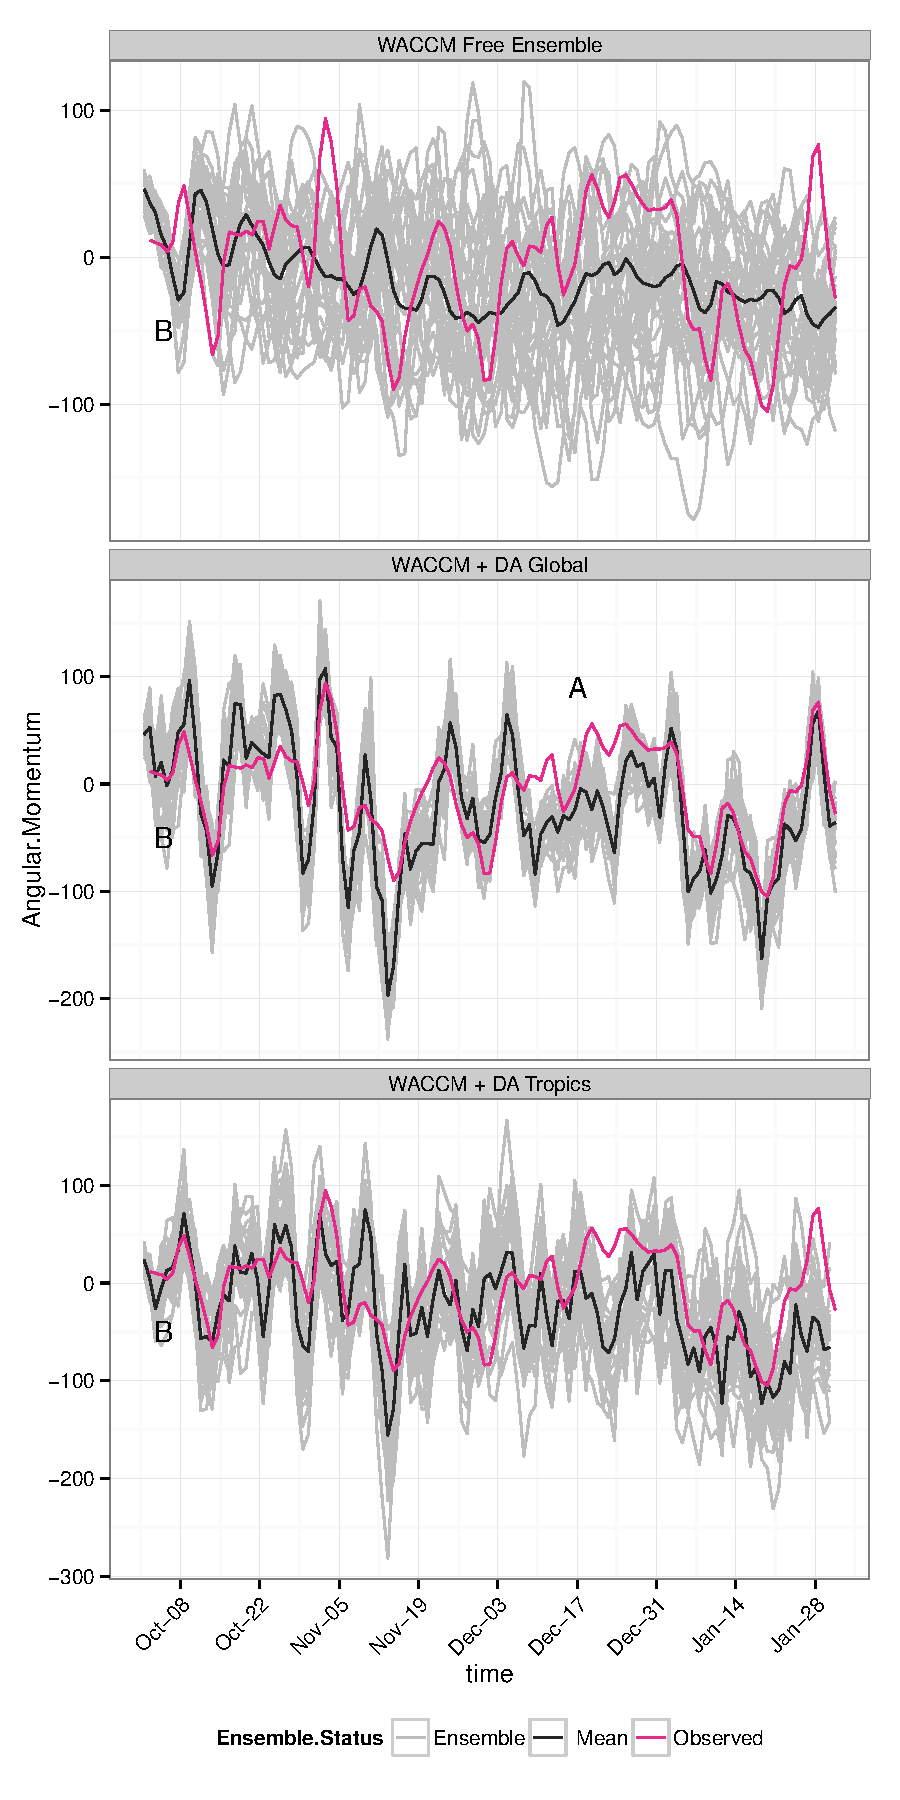
\includegraphics[width=0.5\textwidth]{Paper_figures/ERPDA_paper_evalvariable_aam_space_X2only.pdf}
	 \caption{Comparison of the ensemble (gray) and its mean (black) in DART-WACCM experiments with increasing observational constraints (Table \ref{tab:expts}), in terms of angular momentum excitation functions $\chi_2$ and $\chi_3$ Each angular momentum function is compared to the angular momentum implied by the corresponding Earth rotation parameters (pink).}
	 \label{fig:evalvariable_aam}
\end{figure}
